\documentclass[m,binding,scrreprt,master,palatino]{WeSTthesis}
%\documentclass[m,binding,twoside,scrreprt,master,palatino]{WeSTthesis}
\usepackage[english,ngerman]{babel}		% English and new German spelling
\usepackage[utf8]{inputenc}           % correct input encoding
\usepackage[T1]{fontenc}              % correct output encoding
\usepackage{graphicx}					      	% enhanced support for graphics
\usepackage{tabularx}				      		% more flexible tabular
\usepackage{amsfonts}					      	% math fonts
\usepackage{amssymb}					      	%	math symbols
\usepackage{amsmath}					      	% overall enhancements to math environment
\usepackage[textsize=footnotesize,textwidth=27.5mm]{todonotes}					      	% package for notes/comments
\usepackage[bookmarks=true,
bookmarksopen=true,
bookmarksnumbered=true,
pdfstartpage=1,
%TODO add final title
pdftitle={},
pdfauthor={Martin Christian Körner},
pdfsubject={Master's Thesis},
%TODO add keywords
pdfkeywords={},
breaklinks=true,
colorlinks=true,
%linkcolor=black,
%anchorcolor=black,
%citecolor=black,
%filecolor=black,
%menucolor=black,
%urlcolor=black]{hyperref}
linkcolor=blue,
anchorcolor=blue,
citecolor=blue,
filecolor=blue,
menucolor=blue,
urlcolor=blue]{hyperref}
\usepackage{float}                    % additional positions for images
\usepackage{listings}                 % source code
\usepackage[font=bf,labelfont=bf]{caption}    % captions
\usepackage{appendix}                 % appendix
\usepackage{microtype}
\usepackage{multirow}% http://ctan.org/pkg/multirow
\usepackage{epstopdf}
\usepackage[capitalize,noabbrev,nameinlink]{cleveref} % for \Cref
\usepackage[toc,nonumberlist,acronym]{glossaries} % make a separate list of acronyms
\usepackage{bm}
\usepackage{bbm}
\usepackage{scrhack}
\usepackage[style=alphabetic,hyperref=true,backref=true,natbib=true,abbreviate=false]{biblatex}



\newcommand{\itodo}[1]{\todo[inline]{#1}}

%TODO add matriculation number to WeSTthesis.cls?
\author{Martin Körner\\[0.1cm]\normalsize{Matrikelnummer: 210200113}\vspace{-0.5cm}}

\title{Reference String Extraction from\\
Social Science Research Papers using\\
Conditional Random Fields and\\
Distant Supervision}

\degreecourse{Web Science}

\firstreviewer{Prof. Dr. Steffen Staab}
\firstreviewerinfo{Institute for Web Science and Technologies}

\secondreviewer{Ren\'e Pickhardt}
\secondreviewerinfo{Institute for Web Science and Technologies}

% load globally defined glossaries
\loadglsentries{/home/martin/glossaries/mathematics/probability-theory/graphical-models/glossary.tex}
\loadglsentries{/home/martin/glossaries/mathematics/probability-theory/glossary.tex}
\loadglsentries{/home/martin/glossaries/mathematics/graph-theory/glossary.tex}
\loadglsentries{/home/martin/glossaries/mathematics/glossary.tex}

% load local glossary
\loadglsentries{frontbackmatter/glossary.tex}

% load local acronyms
\loadglsentries{frontbackmatter/acronyms.tex}


% use italics for the first use of a glossary term
\defglsdisplayfirst[\glsdefaulttype]{\textit{#1}}

\makeglossaries

\addbibresource{frontbackmatter/bibliography.bib}

\begin{document}
\pagenumbering{roman}

\maketitle

\begin{center}
  \begin{large}
  \bfseries{Zusammenfassung}
  \end{large}
\end{center}
Zusammenfassung auf Deutsch
\par\bigskip
\par\bigskip
\selectlanguage{english}
\begin{center}
  \begin{large}
  \bfseries{Abstract}
  \end{large}
\end{center}
To help in overcoming a shortage of citation information for the German social sciences, we contribute an approach for extracting author names from reference sections.
Instead of relying on small amounts of manually labeled data, we use a distantly supervised approach to automatically generate a partially labeled training data set.
To apply this data set to the widely used probabilistic framework of conditional random fields, GE criteria provide a suitable objective function.
The resulting model does not only decide if a word is part of an author, but also separates the listed authors and distinguishes between first and last names.
The evaluation of our model reports a promising performance for the author extraction task.
In addition, it suggests ways of influencing the trade-off between the precision and recall of the model.

\varclearpage

%TODO add license
%\begin{center}
\includegraphics{figures/cc-by-sa.eps}
\end{center}
\begin{small}
This work is licensed under the Creative Commons Attribution-ShareAlike 4.0 International License. To view a copy of this license, visit \url{http://creativecommons.org/licenses/by-sa/4.0/}.
\end{small}

%\varclearpage

\tableofcontents
\varclearpage

\pagenumbering{arabic}
% list of figures
% \listoffigures
% \varclearpage

% beginning of the actual text section
%\listoftodos
\clearpage
\chapter{Introduction}\label{cha:introduction}

% What is the thesis about?
% Why is it relevant or important?
% What are the issues or problems?
% What is the proposed solution or approach?
% What can one expect in the rest of the thesis?


Citation data provides information on which scholarly work cites with other scholarly work.
This information is essential for the knowledge discovery process when conducting research and there are several services available that provide citation data for research areas like mathematics and physics\footnote{\url{http://related-work.net/}}, computer science\footnote{\url{http://dblp.uni-trier.de/}}, and medicine\footnote{\url{http://www.ncbi.nlm.nih.gov/pubmed}}.
Despite its importance, there is a shortage of citation data for German social science research papers~\cite{herb2015open}.
Even though there are commercial services available which provide citation data for a broad range of research areas, they do not provide a sufficient coverage of smaller academic fields like the German social sciences.
This could be explained by the low profitability of including such data.
In addition, commercial services generally do not publicly share their dataset which hinders a full utilization of the citation data.
The Social Science Citation Index\footnote{\url{http://scientific.thomson.com/products/ssci/}} by Thomson Reuters in particular was criticized for being ideologically biased and containing methodological deficiencies in the citation counting~\cite{klein2004social}.
Thereby, the motivation of this thesis is to contribute to the effort of extracting citation data from given research papers in order fill the gap regarding the German social sciences and to be less dependent on commercial services.

\bigskip

The different steps for extracting citation data from PDF documents are shown in \todo{add}.
At first the content of the PDF files is converted to text files to allow easier processing.
In the second step the reference strings are extracted from the text.
The strings are then segmented into the different attributes that identify the referenced paper (step three).

Such attributes can be the authors, title, journal, and publication year.
This information then needs to be matched against existing meta data records in order to assign a unique identifier such as a \gls{doi} to the reference (step four) to generate a citation network.
This thesis has not the goal of covering the whole pipeline.
Instead, we focus on the extraction reference strings from a given article in plain text.

\itodo{clarify/define reference vs citation}

The implementations that result from thesis are available on \todo{link} under a open-source license.


The remainder of this thesis is structured as follows.
In \Cref{cha:introduction} we introduce the problem of reference string extraction and in particular the extraction of author names in references.



\varclearpage
\chapter{Related Work}\label{cha:related-work}
In this chapter we will give an overview of the related work in the area of information extraction from research papers.
We will also survey \gls{distant supervision} as a method for generating training data without manual labeling.

\bigskip

There has been a large body of research on information extraction from research papers and in the following we discuss a number of examples for such research.

\citet{giles1998citeseer} propose one of the first autonomous citation indexing systems called \emph{CiteSeer}.
It converts papers that are extracted from the World Wide Web to text, extracts the references and the context in which they are made in the body of the paper, and stores the information in a database.
Yet, the extraction happens based on simple heuristics which results in a relatively low accuracy compared to more advanced approaches.
In an evaluation of \num{5093} documents related to ``neural networks'', $80.2\%$ of the titles, $82.1\%$ of the authors, and $44.2\%$ of the page numbers were extracted correctly from the retrieved references~\cite{giles1998citeseer}.

%In order to simplify the creation of personal digital libraries, \citet{marinai2009metadata} proposes a software that combines \gls{pdf} parsing, low level document image processing, and layout analysis.
%First, text blocks of the research paper are segmented and annotated with layout information such as the position on the page and the width and height of the text block.
%Then, a \gls{mlp} classifier is applied on the annotated text blocks in order to extract the title and authors of the research paper.
%Based on this pair of title and authors, additional information about the paper is extracted from the DBLP\footnote{\url{http://dblp.uni-trier.de/}} computer science bibliography.
%Evaluated on 80 papers, the approach of learning from layout information resulted in successfully extracting 95\% of the titles and, by integrating information from DBLP, 73.58\% of the authors.

\citet{powley2007evidence} address both citation extraction and citation-reference matching in research papers.
For the citation extraction, they achieved a very high precision ($99.88\%$) and recall ($96.78\%$) by identifying pairs of year and author surnames in the text.
The citation-reference matching was done in an integrated fashion.
A plain text representation of the reference section was segmented into reference strings by matching the author and year information form the extracted citation data.
This approach again resulted in a very high precision and recall for both the reference segmentation and citation-reference matching \citep{powley2007evidence}.

For extracting bibliographic attributes from research papers that are only available as images, \citet{takasu2003bibliographic} uses optical character recognition combined with a variation of \glspl{hmm}.
The evaluation was based on \num{1,575} references obtained from Japanese journal papers and the reported accuracy was above $90\%$ for all extracted bibliographic attributes except the volume and volume number.

%TODO extend this:
Instead of using \glspl{hmm}, \citet{peng2004accurate}, \citet{councill2008parscit}, as well as \citet{groza2012reference} rely on \glspl{crf} for extracting bibliographic information from research papers.
The three approaches followed the same steps:
After extracting and segmenting the reference strings, they are split into tokens and each token gets assigned a number of features.
Example for such features are the position in the line, whether or not the token starts with a capitalized letter, contains a dot, or only contains digits.
In addition, external lexicons are used in order to determine features like (author) surnames, places, and months.
The \gls{crf} is learned on data set containing between 200 and 830 references where every element of the reference gets analyzed for the set of features and also manually assigned a label such as author, title, year, and publisher.
The trained \gls{crf} is then used for labeling unseen testing data and the performance is evaluated using precision, recall, and the $\text{F}_1$ score.
\citet{groza2012reference} give an overview of the results of the three mentioned studies on the so-called CORA dataset which contains $200$ reference strings.
The results show a very promising performance with $\text{F}_1$ scores higher than $93\%$ for all labeled element types and with an average of $96.7\%$ \citep{groza2012reference}.

Regarding the extraction of the reference string from a given research paper, \citet{councill2008parscit} as well as \citet{groza2012reference} relied on regular expressions that search for section labels like ``References'' or ``Bibliography'' and regarded the following text as reference strings.
Other regular expressions were used to identify a section heading that ends the reference  block such as ``Appendix'', ``Acknowledgments'', or the end of the document.
The content of the extracted reference block was separated into reference strings with another set of regular expressions that search for makers like ``[1]'', ``[PM04]'', or ``1.'' at the beginning of the lines.
If such markers were not found, other heuristics like author names at the beginning of the line, punctuation at the end of the line, and the length of the line were used.
This approach was sufficient for the considered use cases in computer science and health sciences \citep{councill2008parscit,groza2012reference}.
Other related studies such as the one by \citet{peng2004accurate} did not retrieve reference strings from research papers but used a preprocessed data set containing reference strings.

\bigskip

\citet{mintz2009distant} propose the paradigm of \gls{distant supervision} for relation extraction to avoid the weaknesses of supervised, unsupervised, and bootstrap learning.
They argue that supervised learning can only be done with small data sets since labeling data manually is expensive.
Purely unsupervised information extraction on the other hand may result in findings that are unrelated to a particular knowledge base \citep{mintz2009distant}.
The third approach, bootstrap learning on a small number of seed instances, is said to often suffer from low precision and semantic drift \citep{mintz2009distant}.
By using an external source of information for the supervision, \gls{distant supervision} is able to train on large amounts of data without loosing the focus on the relevant knowledge base \citep{mintz2009distant}.
In their use case of relation extraction, \citet{mintz2009distant} use the semantic database \gls{freebase} \citep{bollacker2008freebase} for the \gls{distant supervision}.
The assumption is that if a sentence contains a pair of entities that are part of a \gls{freebase} relation, it is likely to express that relation in some way \citep{mintz2009distant}.
A human evaluation of the extracted relations resulted in a $67.6\%$ precision.

\citet{fan2015detecting} apply the concept of \gls{distant supervision} to the detection of tables in \gls{pdf} files.
Their assumption is that tables in research papers have surrounding captions that conform to a limited number of official templates \citep{fan2015detecting}.
Following this assumption, a training set is automatically generated by extracting the context around text lines that start with words like ``Table'' or ``Tab.''.
The extracted context also includes further information about the coordinates in the file and the font style \citep{fan2015detecting}.
Three canonical classifiers, namely Logistic Regression, Support Vector Machines, and Naive Bayes, are built with the training set \citep{fan2015detecting}.
Their performance was evaluated against a \emph{Heuristics} approach \citep{klampfl2014comparison} that was assumed to be state-of-the-art.
The evaluation on two data sets showed that the approach by \citet{fan2015detecting} was superior to the Heuristics approach in all cases.

\itodo{\citet{lu2013web}: distant supervision and GE on name entity recognition}

\bigskip

In summary, several aspects of the information extraction from research papers can be achieved with a considerably good performance.
Especially the segmentation of a given reference string into its elements by using \glspl{crf} \citep{peng2004accurate,councill2008parscit,groza2012reference} as well as the combination of citation extraction and citation-reference matching \citep{powley2007evidence} show very promising results.
Yet, all current approaches have in common that they rely on manually labeled data sets for training their models.
Manually labeled data sets are expensive and thereby usually only exist in smaller quantities.
In our particular use case of extracting references from German social science research papers, no such data set is currently available.

\Gls{distant supervision} is a promising approach that allows the reduction of labeling costs by including external sources of information during the generation of partially annotated data sets.

In order to use such a data set for the training of a \gls{crf} model, two approaches were discussed.
\citet{tsuboi2008training} marginalize unlabeled tokens by generating sequences for all possible labelings for these tokens.
Instead of labeled instances, \citet{mann2008generalized} use \gls{ge} criteria and labeled features.
In addition they can also incorporate \glspl{conditional probability distribution} over the labelings.

In the following chapter we will first introduce \glspl{crf} as a framework for modeling \glspl{probabilistic graphical model}.
This will build the foundation of our discussion in \Cref{cha:distant-supervision} about the usage of partially annotated data in \glspl{crf} during \gls{distant supervision}.


\varclearpage

\chapter{Distant Supervision}\label{cha:distant-supervision}

A common approach to the learning of \glspl{crf} is to use manually labeled instances.
Manual labeling results in an accurate labeling in most cases but is expensive and can thereby only be performed on small data sets.

%TODO general words on distant supervision: jiang2012information

The approach of \gls{distant supervision} allows the automated labeling of large data sets by using heuristics and external sources of information.

In this chapter we will first give an overview of \gls{distant supervision} by discussing the past usages.
We will then discuss approaches on how \glspl{crf} can be learned using distantly supervised data sets.

\section{Overview}

%TODO explain origin
Before explaining our usage of the term \gls{distant supervision}, we will first examine its origin and how it was previously used.

\bigskip

As discussed in \Cref{cha:related-work}, the term \gls{distant supervision} was introduced by \citet{mintz2009distant} as an approach for relation extraction without labeled data.
They state that \gls{distant supervision} extends the paradigm used by \citet{snow2005learning} for the extraction of hypernyms.
This is done by learning dependency paths from hypernym/hyponym word pairs that were extracted from WordNet~\citep{snow2005learning}.
The dependency paths are then used as features in a logistic regression classifier with the task of identifying hypernym pairs in a corpus~\citep{snow2005learning}.
Additionally, \citet{mintz2009distant} mention a similarity of \gls{distant supervision} to the usage of weakly labeled data in bioinformatics.
One mentioned example is how \citet{craven1999constructing} extract relations between biological objects such as proteins, cell-types, and diseases from a text corpus.
For this they train a Naive Bayes classifier with data from the Yeast Protein Database~\citep{payne1997yeast}.
\citet{surdeanu2012multi} go as far as saying that distant supervision for \gls{ie} was introduced by \citet{craven1999constructing}.

While not giving a definition of the term, \citet{mintz2009distant} state that ``[t]he intuition of distant supervision is that any sentence that contains a pair of entities that participate in a known Freebase relation is likely to express that relation in some way.''

There is now a body of research that uses the paradigm of \citet{mintz2009distant} for relation extraction~\citep{benson2011event,ritter2011named,nguyen2011end,takamatsu2012reducing,xu2013filling}.

\bigskip

Another intuition of \gls{distant supervision} that is not based on leveraging existing knowledge bases such as FreeBase.
\citet{go2009twitter} use emoticons in Twitter\footnote{\url{https://twitter.com/} (accessed May~19,~2016)} tweets as noisy labels to build the training set for sentiment analysis~\citep{go2009twitter}.

There is again a body of research that extends this approach to sentiment analysis~\citep{purver2012experimenting,marchetti2012learning,suttles2013distant}.

\citet{fan2015detecting} also apply distant supervision without using a knowledge base.
They rely on a simple heuristic for localizing tables by considering the context around a line starting with ``Table'' or ``Tab.'' as a potential table.

%TODO ling2012fine on entity recognition using distant supervision
\bigskip

Due to the different applications of \gls{distant supervision}, a precise definition\dots

What all approaches have in common is that they use some heuristic to assign labels to previously unlabeled data. These labelings are are used during the training, either in addition to preexisting labeled data or on their own.



\section{Distant Supervision and \glsentryshortpl{crf}}

Data sets that are used within a distantly supervised learning approach are typically incompletely annotated.
This is due to the fact that, in practice, external knowledge bases can not cover all observed cases in the training set.
As a result, conventional \gls{crf} learning algorithms cannot be directly applied to such data sets since they require a fully annotated input~\citep{tsuboi2008training}.

To make this more clear, recall that for \glspl{crf} we have $\bm{D}_k\not\subseteq\bm{X}$ for every $k=1,\dots,K$ (see \Cref{sec:definition-crfs}).
In other words, every set of \glspl{random variable} $\bm{D}_k$ needs to contain at least one $Y_n\in\bm{Y}$.
Otherwise, the term containing $\bm{D}_k$ cancels out during the calculation of $P(\bm{Y}\mid\bm{X})$ due to the normalization constant $Z(\bm{X})$ (see \todo{add ref} for an example).
Thereby the question arises on how data sets are handled where not every element is labeled.

In this section we will discuss approaches that use incompletely annotated data for the learning of \glspl{crf}.
\itodo{sentence on tsuboi approach?}
A very promising approach, especially for our author extraction use case (see \Cref{cha:author-extraction}), is \gls{ge}, proposed by \citet{mann2007simple}.

\subsection{Marginalization}
%TODO \citet{tsuboi2008training}: problems with absolute input
%TODO instead: add the same prob distr. to all unknown tags?
\citet{tsuboi2008training} propose a method of training \glspl{crf} using incomplete annotations.
They consider two cases of incomplete annotations: Partial and ambiguous annotations.
By considering all possible label sequences that are with a given incomplete labeled sequence, it is possible to marginalize the unknown labels out.
Yet, the resulting equations is not a concave function which prevents efficient global maximization~\citep{tsuboi2008training}.
Instead, they rely on gradient ascent iterations which were proposed by~\citep{sha2003shallow}.
Another challenge that arises is the amount of label sequences that are generated this way which is exponential in the number of unknown labels~\citep{tsuboi2008training}.
This problem is addressed by applying the Markov assumption and using a modification of the Forward-Backward algorithm~\citep{tsuboi2008training}.
\citet{tsuboi2008training} apply their approach on Japanese word segmentation using partial annotations and on \gls{pos} tagging using ambiguous annotations.
For the word segmentation task the proposed approach was compared with two other methods that can handle partial annotations.
The first one is filling unknown labels by prediction based on the partial annotations and the second one is training a point-wise classifier that excludes label correlations~\citep{tsuboi2008training}.
The reported results show that the proposed method outperforms both methods for various sample sizes.
For the \gls{pos} tagging they used the Penn treebank corpus \citep{marcus1993building} which contains a number of ambiguous \gls{pos} tags.
The proposed approach was compared with three other heuristics, namely random selection, selecting the first tag in the description order, and selecting the most frequent tag in the corpus.
In this case, the proposed method only moderately improved the performance which the authors believe it due to the relatively low percentage of ambiguous tags in the corpus~\citep{tsuboi2008training}.

\subsection{Generalized Expectation (\glsentryshort{ge})}

Instead of ``filling the gaps'' of incomplete annotations, \citet{mann2008generalized} apply the concept of \gls{ge} on the training of linear-chain \glspl{crf}.
\Gls{ge} was first proposed in \citet{mann2007simple} under the name \gls{expectation regularization} as a method for semi-supervised learning.
%TODO definition GE

\citet{mann2008generalized} use \gls{ge} criteria to train \glspl{crf} on labeled features instead of fully labeled instances.
More precisely, the \gls{ge} criteria are used as an additional regularization term in the log-likelihood function during the model learning.

%TODO define \mathcal{U}
In general, a \gls{ge} criterion $G(\bm{\theta};\mathcal{U})$ is a score function $S$ which is defined as~\citep{mann2010generalized}
\begin{equation}
  \label{equ:generalized-expectation}
  G(\bm{\theta};\mathcal{U})=S\left(E_{\mathcal{U}}\left[E_{P(\bm{Y}\mid\bm{X})}\left[G(\bm{X},\bm{Y})\right]\right]\right)
\end{equation}

In the following we will consider $\tilde{P}$ to be a \gls{crf} based on the model $\tilde{\mathcal{M}}=\{\tilde{\mathcal{K}},\bm{\tilde{\theta}}\}$.

%target distribution: distribution for every constraint?
%expectations: calculated for every constraint separately (mallet code)?


\itodo{example}
One advantage is that it requires only the labeling of a number of occurrences of a feature in the data set instead of a full annotation.
Additionally, \gls{ge} criteria can take \glspl{conditional probability distribution} of labels given a feature as an input in order to train a model that matches this distributions \citep{mann2008generalized}.

\bigskip

%TODO objective function in mann2008 (and in mallet) is calculated with GE+gaussian prior instead of log-likelihood+gaussian prior+GE

\varclearpage


%\appendix
%\appendixpage
%\addappheadtotoc
%\input{appendices/insert-filename-here}
%\varclearpage


\printglossary[style=altlist]
\printglossary[type=\acronymtype]
%\printglossaries

%\bibliographystyle{plain}
%\bibliographystyle{alpha}

\printbibliography
\varclearpage

%\input{danksagung}
\end{document}
